% !TEX encoding = IsoLatin
% !TEX TS-program = pdflatex

\documentclass[traditabstract]{aa}
\input Planck.tex

% This is useful to overcome a bug in some versions of
% Adobe Acrobat for Windows
\pdfminorversion=4

\usepackage[breaklinks,colorlinks,citecolor=blue]{hyperref}
\usepackage{amsmath}
\usepackage{natbib}
\usepackage{graphicx}
\usepackage{txfonts}
\usepackage{natbib}

\newcommand{\sometext}{\Planck text text text text text text text text text text text text text text text text text text text text text text text text text text text text text text text text text text text text text text text text text text text text text text text text text text text text text text text text text text text text text text text text text text text text text text text text text text text text text text text text text text text text text text text text text text text text text text text text text text text text text text text text text text text text text text text text text text text text text text text text text text text text text text text text text text text text text text text text text text text text text text text text text text text text text text text text text text text text text text text text text text text text text text text text text text text text text text text text text text text text text text text text text text text text text text text text text text text text text text text text text text text text text text text text text text text text text text text text text text text text text text text text text text text text text text text text text text text}

\bibpunct{(}{)}{;}{a}{}{,}

\begin{document}

\title{P00: Planck Paper Plots}

\author{
	Zonca, A. \inst{1}
}

\institute{UCSB\\
	\email{zonca@deepspace.ucsb.edu}
}

\date{\today}

\abstract{Abstract abstract abstract abstract abstract abstract abstract abstract abstract abstract abstract abstract abstract abstract abstract abstract abstract abstract abstract abstract abstract abstract abstract abstract abstract abstract abstract abstract abstract abstract abstract abstract abstract abstract abstract abstract abstract abstract abstract abstract abstract abstract abstract abstract abstract abstract abstract abstract abstract abstract abstract abstract abstract abstract abstract abstract abstract abstract abstract abstract abstract abstract abstract abstract abstract abstract abstract abstract abstract abstract abstract abstract abstract abstract abstract abstract abstract abstract abstract abstract abstract abstract abstract abstract abstract abstract abstract abstract abstract abstract abstract abstract abstract abstract abstract abstract abstract abstract abstract abstract abstract abstract}

\keywords{cosmic microwave background -- Instrumentation: polarimeters -- Methods: data analysis}

\maketitle

%%%%%%%%%%%%%%%%%%%%%%%%%%%%%%%%%%%%%%%%%%%%%%%%%%%%%%%%%%%%%%%%%%%%%%

\section{Power spectrum}

\sometext

\begin{figure}[h]
\centering
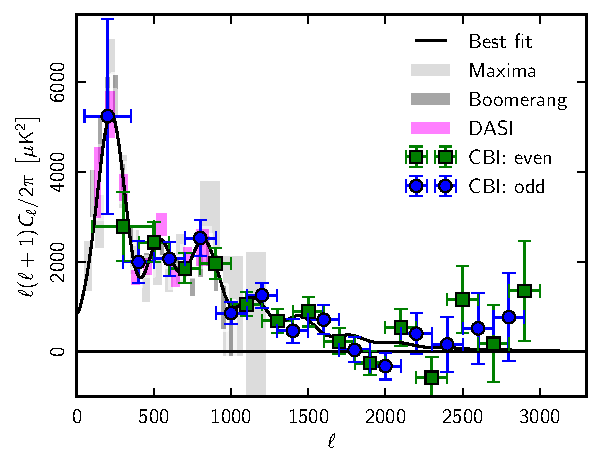
\includegraphics[width=8.8cm]{powerspectrum_88mm.pdf}
\caption{\label{fig:gainCurve} 8.8cm wide} 
\end{figure}

\sometext

\begin{figure*}[h]
\centering
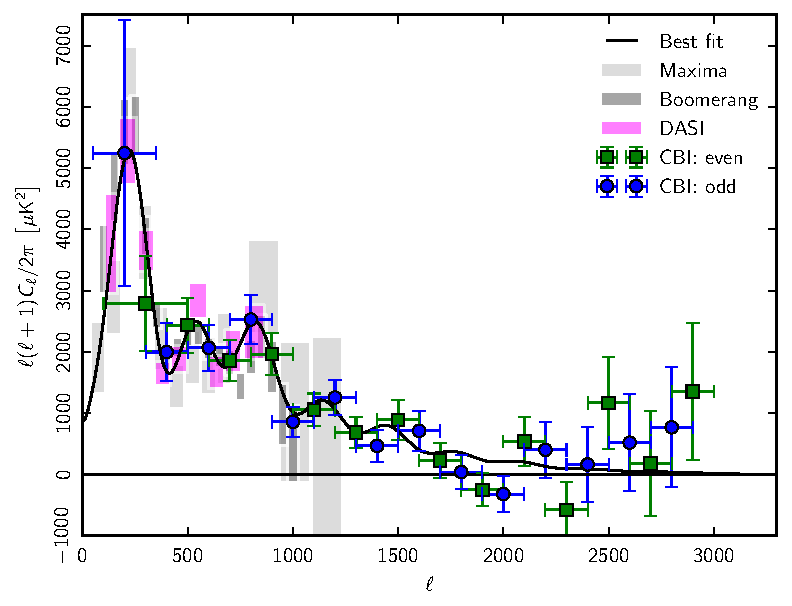
\includegraphics[width=12cm]{powerspectrum_120mm.pdf}
\caption{\label{fig:gainCurve} 12cm wide} 
\end{figure*}

\begin{figure*}[t]
\centering
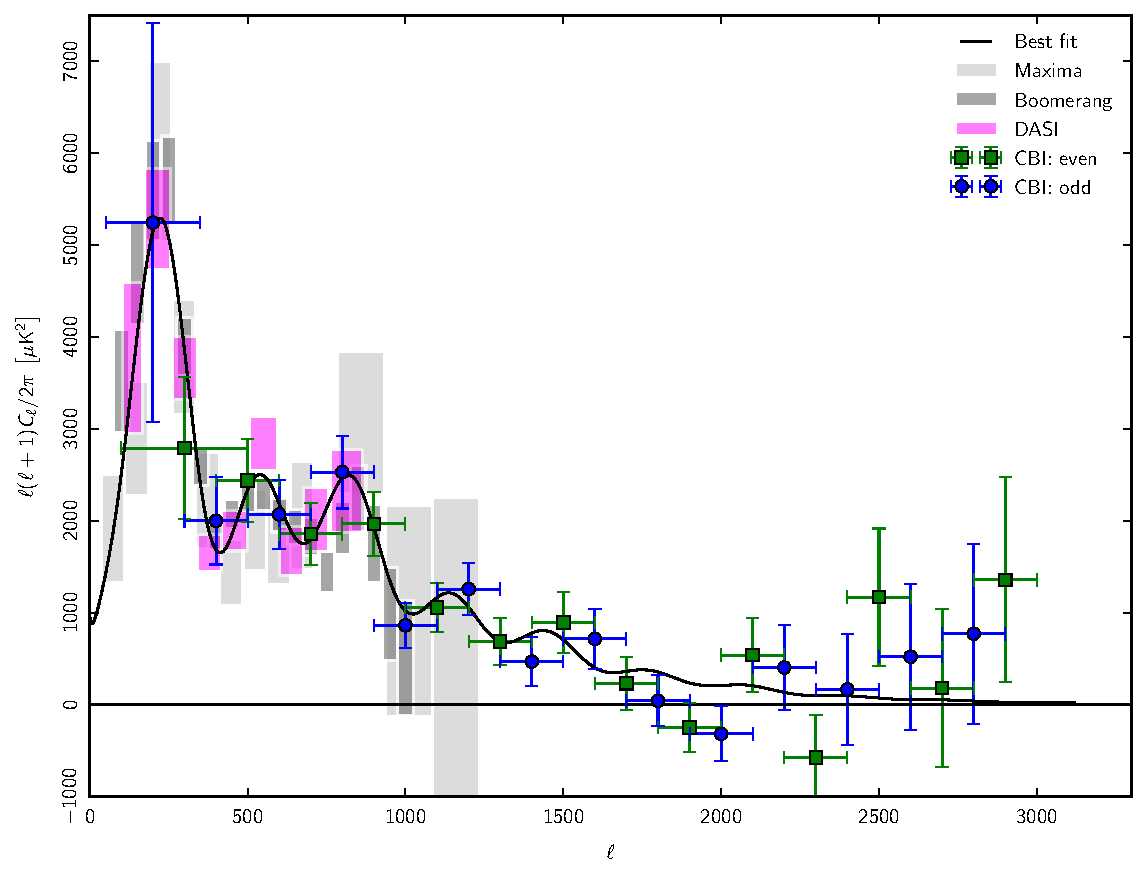
\includegraphics[width=18cm]{powerspectrum_180mm.pdf}
\caption{\label{fig:gainCurve} Figure created at 18cm wide and setting  width=18cm in includegraphics}
\end{figure*}

\clearpage

\section{Mollview}

\sometext

\begin{figure}[h]
\centering
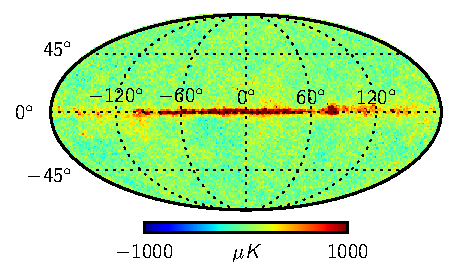
\includegraphics[width=8.8cm]{mollview_88mm}
\caption{\label{fig:gainCurve} 8.8cm wide} 
\end{figure}

\sometext

\sometext

\sometext

\begin{figure*}[h]
\centering
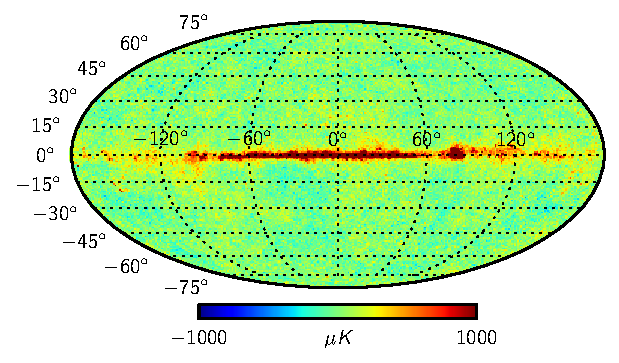
\includegraphics[width=12cm]{mollview_120mm}
\caption{\label{fig:gainCurve} 12cm wide} 
\end{figure*}


\begin{figure*}[H!b]
\centering
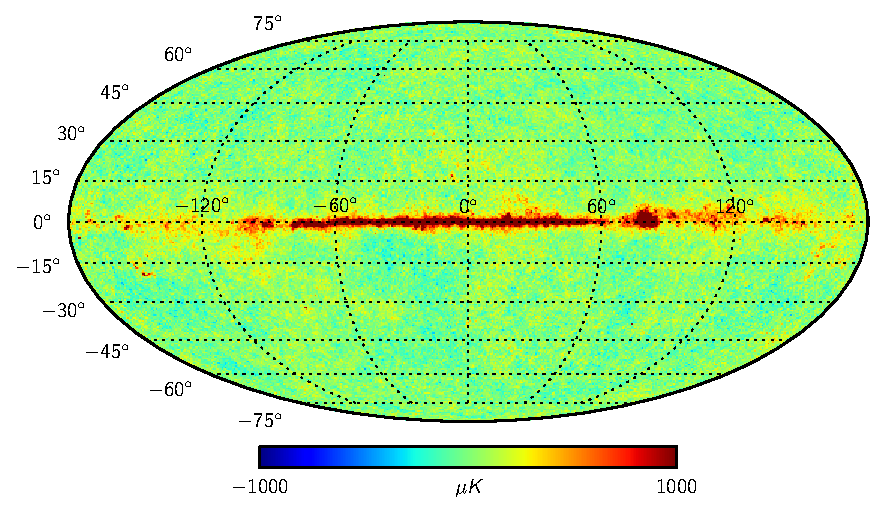
\includegraphics[width=18cm]{mollview_180mm}
\caption{\label{fig:gainCurve} Mollview}
\end{figure*}


\begin{figure*}[H!b]
\centering
\includegraphics[width=17cm]{params}
\caption{\label{fig:gainCurve} Parameters}
\end{figure*}

\end{document}
